\documentclass[12pt]{article}
\usepackage[margin=1in]{geometry}
\usepackage{amsmath}
\usepackage{amssymb}
\usepackage{amsfonts}
\usepackage{amsthm}
\newtheorem{thm}{Theorem}[section]
\newtheorem{cor}[thm]{Corollary}
\newtheorem{lem}[thm]{Lemma}
\usepackage{tikz}
\usepackage{tikz-cd}
\renewcommand{\d}{\mathrm{d}}

\begin{document}

\title{Math 180 Homework 2}
\author{Nathan Solomon}
\maketitle

\textbf{Due January 26th}

\section{}
\noindent\fbox{\fbox{\parbox{6.5in}{
    Draw the following graphs:
    \begin{itemize}
        \item (1) The claw graph $C = (\{1,2,3,4\}, \{a,b,c\}, \varphi)$ where $\varphi$ is given by
        \begin{center}
            \begin{tabular}{|c|c|c|}
                \hline
                $a$ & $b$ & $c$ \\
                \hline
                $\{1,2\}$ & $\{1,3\}$ & $\{1,4\}$ \\
                \hline
            \end{tabular}
        \end{center}
        \item (2) The paw graph $P = (\{1,2,3,4\}, \{a,b,c,d\}, \varphi)$ where $\varphi$ is given by
        \begin{center}
            \begin{tabular}{|c|c|c|c|}
                \hline
                $a$ & $b$ & $c$ & $d$\\
                \hline
                $\{1,2\}$ & $\{1,3\}$ & $\{1,4\}$ & $\{2,3\}$ \\
                \hline
            \end{tabular}
        \end{center}
        \item (3) The bull graph $B = (\{1,2,3,4,5\}, \{a,b,c,d,e\}, \varphi)$ where $\varphi$ is given by
        \begin{center}
            \begin{tabular}{|c|c|c|c|c|}
                \hline
                $a$ & $b$ & $c$ & $d$ & $e$ \\
                \hline
                $\{1,2\}$ & $\{1,3\}$ & $\{1,4\}$ & $\{2,3\}$ & $\{2,5\}$ \\
                \hline
            \end{tabular}
        \end{center}
    \end{itemize}
}}}\bigskip\par
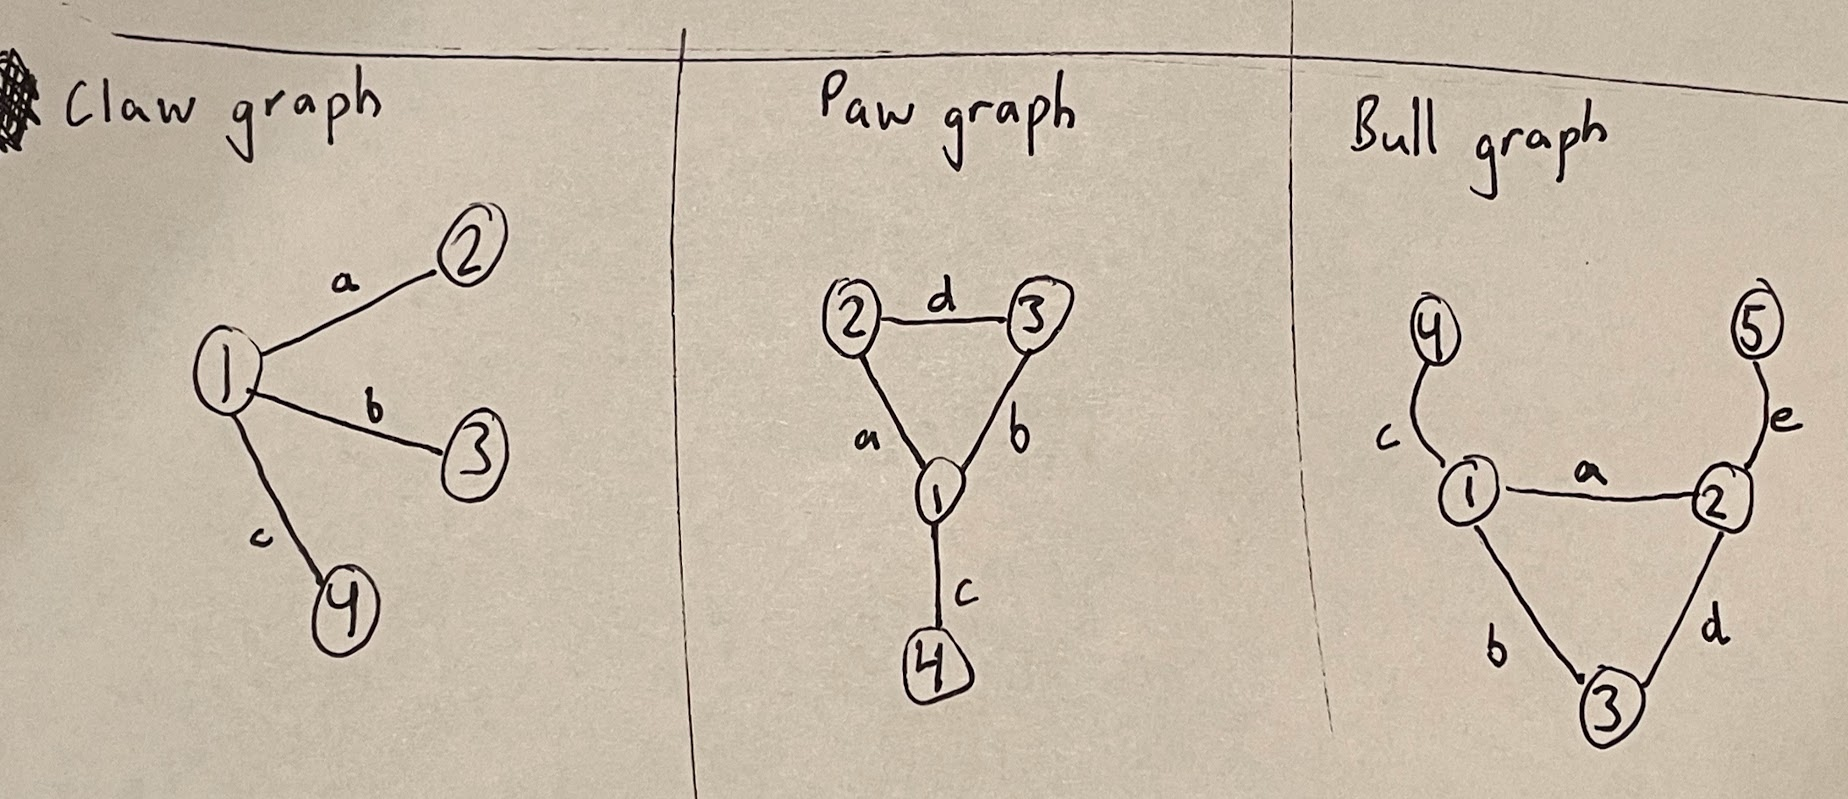
\includegraphics[width=\textwidth]{IMG_1384.jpg}

\section{}
\noindent\fbox{\fbox{\parbox{6.5in}{
            \textbf{Section 4.1, exercise 1}
}}}\bigskip\par
\begin{itemize}
    \item (a) See the vertex labels below. There exists a function which takes each vertex in the graph on the left and maps it to the vertex with the same label in the graph on the right. In either graph, vertices are connected by an edge if and only if the sets they're labeled with do not have any overlap. Since the function I just described preserves that property, two vertices in the graph on the left are connected by an edge if and only if the corresponding vertices in the graph on the right are connected by an edge. This function is an isomorphism between those two graphs.
    \item (b) This property is obvious from looking at either graph. For each of them, the vertex set matches the vertex set in the definition of the Petersen graph, and edges exist between vertices if and only if the definition for the Petersen graph says they should.
\end{itemize}
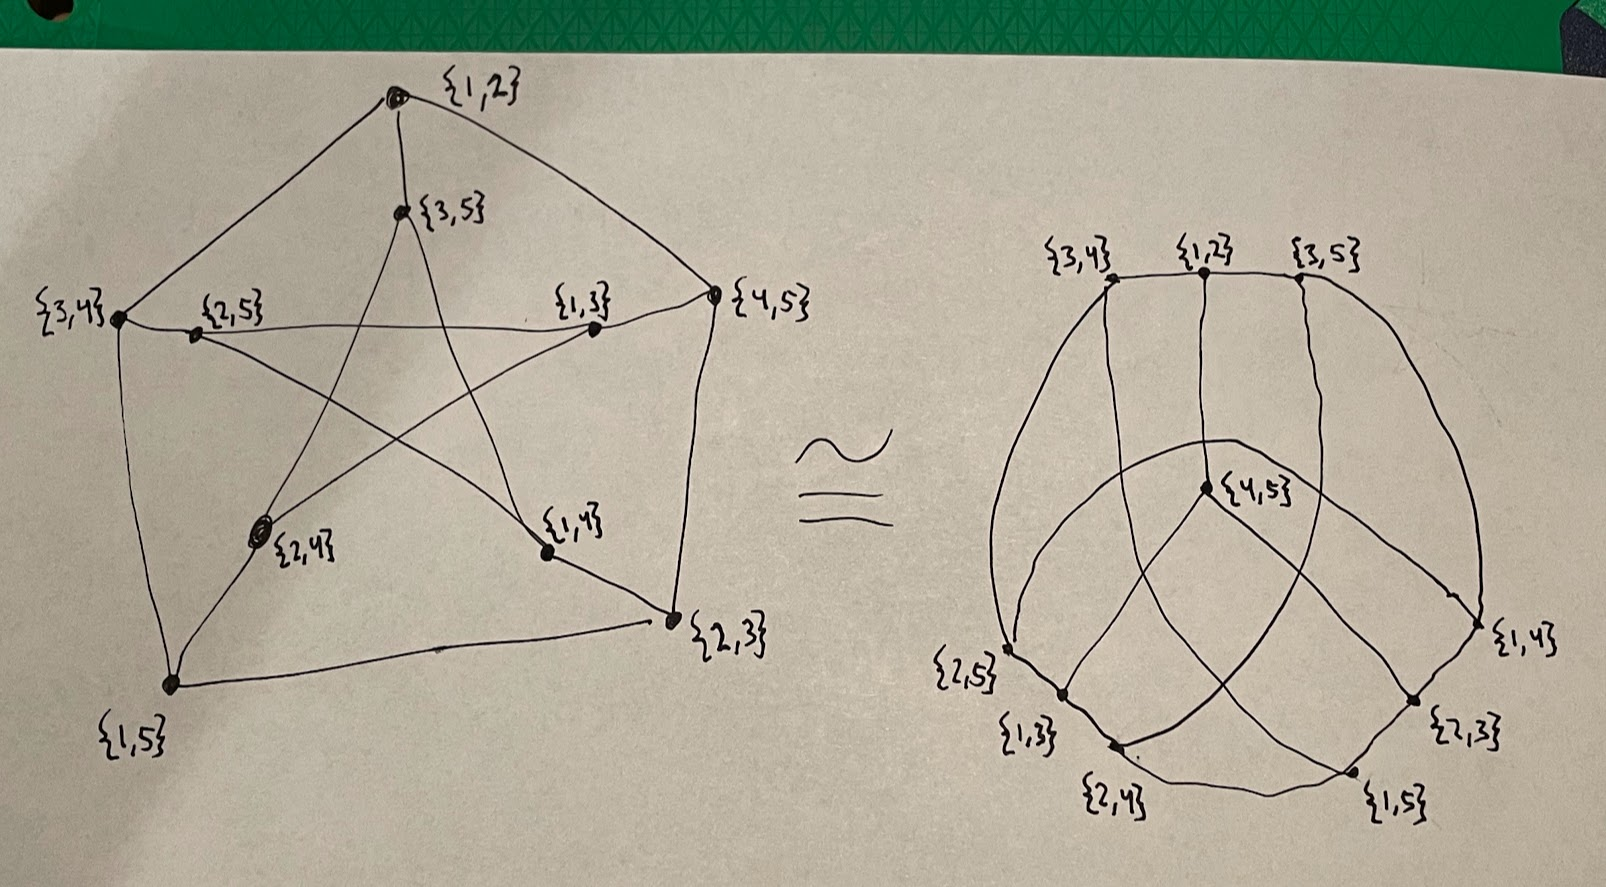
\includegraphics[width=\textwidth]{IMG_1383.jpg}

\section{}
\noindent\fbox{\fbox{\parbox{6.5in}{
    How many automorphisms do the following graphs have?
    \begin{itemize}
        \item (1) $K_n$
        \item (2) $C_n$
        \item (3) $P_n$
    \end{itemize}
}}}\bigskip\par
\begin{itemize}
    \item (1) A graph isomorphism on $K_n$ (the complete graph with $n$ vertices) can be any permutation of the vertices. Every pair of vertices is connected by an edge, and permutating the vertices doesn't change that, so there are no further restrictions on what permutations of vertices are allowed. Therefore tehre are $n!$ graph isomorphisms on $K_n$.
    \item (2) Let $f$ be an automorphism on $C_n$ (the cycle graph with $n$ vertices, assuming $n>2$. Label one of the vertices $a$ and label one of its two adjacent vertices (which are guaranteed to be distinct) $b$. We can build any such $f$ by choosing $f(a)$ to be any of the $n$ vertices, then choosing $f(b)$ to be any of the 2 vertices adjacent to $f(b)$. From those 2 choices, $f$ is uniquely defined, so there are $2n$ automorphisms of $C_n$.
    \item (3) Let $f$ be an automorphism of $P_n$ (the path graph with $n$ nodes, where $n>1$). Let $a$ be the start node and $b$ be the end node. Then either $f(a)=a$ or $f(a)=b$, and knowing what $f(a)$ is is enough to determine the whole function. Therefore there are only 2 automorphisms of $P_n$ (the function which doesn't change it, and the function which reverses it).
\end{itemize}

\section{}
\noindent\fbox{\fbox{\parbox{6.5in}{
            \textbf{Section 4.2, exercise 1}. Prove that the complement of a disconnected graph $G$ is connected. (The \textit{complement} of a graph $G=(V,E)$ is the graph $(V, \binom{V}{2}\backslash E)$.)
}}}\bigskip\par
Let $G$ be a disconnected graph and let $a,b$ be any two vertices in $G$. If there is no path from $a$ to $b$, then they don't share an edge, so in the complement of $G$, they do share an edge. If there is a path in $G$ from $a$ to $b$, then since $G$ is disconnected, there exists a vertex $c$ which has not path to either $a$ or $b$. Therefore in the complement of $G$, there are edges connecting both $a$ and $b$ to $c$, and those 2 edges together form a path from $a$ to $b$. So in either case, $a$ and $b$ are connected in the complement of $G$.

\section{}
\noindent\fbox{\fbox{\parbox{6.5in}{
            \textbf{Section 4.3, exercise 7}. Let $G$ be a graph with 9 vertices, each of degree 5 or 6. Prove that it has at least 5 vertices of degree 6 or at least 6 vertices of degree 5.
}}}\bigskip\par
Let $n$ be the number of vertices of degree 6. The sum of the degrees of each vertices is equal to 2 times the number of edges, so
\[ 6n + 5(9-n) = 2E \]
is an even number. Then $n$ cannot be 4, because if it were, the left hand side would be 49, which is odd. Since $n$ is not 4, either $n$ is at least 5, or $9-n$ is at least 6.

\section{}
\noindent\fbox{\fbox{\parbox{6.5in}{
            \textbf{Section 4.3, exercise 9}. Let $G$ be a graph in which all vertices have degree at least $d$. Prove that $G$ contains a path of length $d$ (not necessarily an induced one).
}}}\bigskip\par
Assume $G$ is a simple graph with at least one vertex. If we do not make this assumption, the statement is not true.
\par
Even with this assumption, the statement we want to prove is false. $C_2$ is an example of a graph in which every vertex has degree 2, but there is no path of length two, because that would require the path to have 3 distinct vertices, and $C_2$ only has two vertices.

\section{}
\noindent\fbox{\fbox{\parbox{6.5in}{
    Prove that graph isomorphism is an equivalence relation.
}}}\bigskip\par
Let $G=(V,E)$, $G'=(V',E')$, and $G''=(V'',E'')$ be any graphs for which there exist isomorphisms $f: V \rightarrow V'$ and $g: V' \rightarrow V''$.
\begin{itemize}
    \item \textbf{Reflexive:} The identity map on $V$ is a graph isomorphism from $G$ to $G$.
    \item \textbf{Symmetric:} Since $f$ is a bijection, it has an inverse $f^{-1}: V' \rightarrow V$, and that function satisfies the criteria to be a graph isomorphism from $G'$ to $G$.
    \item \textbf{Transitive:} The function $g \circ f: V \rightarrow V''$ also satisfies all the criteria to be a graph isomorphism (it's a bijection and it preserves edges).
\end{itemize}
We have shown that (1) any graph is isomorphic to itself, (2) that $G$ being isomorphic to $G'$ implies $G'$ is isomorphic to $G$, and (3) that if $G$ is isomorphic to $G'$ and $G'$ is isomorphic to $G''$, then $G$ is isomorphic to $G''$. Therefore graph isomorphism is an equivalence relation.

\end{document}
